% --------------------------------------------------------------
% This is all preamble stuff that you don't have to worry about.
% Head down to where it says "Start here"
% --------------------------------------------------------------
 
\documentclass[12pt]{article}
 
\usepackage[margin=1in]{geometry} 
\usepackage{amsmath,amsthm,amssymb}
\usepackage[margin=1in]{geometry} 
\usepackage{amsmath,amsthm,amssymb}
\usepackage[english]{babel} 
\usepackage[T1]{fontenc} %escribe lo del teclado
\usepackage[utf8]{inputenc} %Reconoce algunos símbolos
\usepackage{lmodern} %optimiza algunas fuentes
\usepackage{graphicx}
\graphicspath{ {images/} }
\usepackage[urlcolor=blue,colorlinks=true]{hyperref}
\usepackage{makecell}
\usepackage{adjustbox}
\usepackage[justification=centering]{caption}
\usepackage[style=alphabetic]{biblatex}  
\addbibresource{references/papers.bib}  
\setlength{\parindent}{0em} 
 
 
\newcommand{\N}{\mathbb{N}}
\newcommand{\Z}{\mathbb{Z}}
 
\newenvironment{theorem}[2][Theorem]{\begin{trivlist}
\item[\hskip \labelsep {\bfseries #1}\hskip \labelsep {\bfseries #2.}]}{\end{trivlist}}
\newenvironment{lemma}[2][Lemma]{\begin{trivlist}
\item[\hskip \labelsep {\bfseries #1}\hskip \labelsep {\bfseries #2.}]}{\end{trivlist}}
\newenvironment{exercise}[2][Exercise]{\begin{trivlist}
\item[\hskip \labelsep {\bfseries #1}\hskip \labelsep {\bfseries #2.}]}{\end{trivlist}}
\newenvironment{problem}[2][Problem]{\begin{trivlist}
\item[\hskip \labelsep {\bfseries #1}\hskip \labelsep {\bfseries #2.}]}{\end{trivlist}}
\newenvironment{question}[2][Question]{\begin{trivlist}
\item[\hskip \labelsep {\bfseries #1}\hskip \labelsep {\bfseries #2.}]}{\end{trivlist}}
\newenvironment{corollary}[2][Corollary]{\begin{trivlist}
\item[\hskip \labelsep {\bfseries #1}\hskip \labelsep {\bfseries #2.}]}{\end{trivlist}}

\newenvironment{solution}{\begin{proof}[Solution]}{\end{proof}}
 
\begin{document}
 
% --------------------------------------------------------------
%                         Start here
% --------------------------------------------------------------
 
\title{Green Orbital Propulsion System for a Small Satellite}
\author{Christian Molli\`ere}
\maketitle
\newpage

% B1
\section{Reference Case Definition}
\label{chap:reference_case}
Most the orbital propulsion systems used for AOCS tasks don't need to provide a very high amount of $\Delta v$ to the satellite bus. Therefore, lightweight and simple blow-down feed systems (see Figure \ref{fig:blowdown_system}) are usually implemented to supply the propellant to the engines. Usually an injector is used to evenly distribute the fuel within the combustion chamber leading to a pressure loss of $\Delta p_{\text{injector}}$ along the fuel line.\\

\begin{figure}[!h]
	\centering
	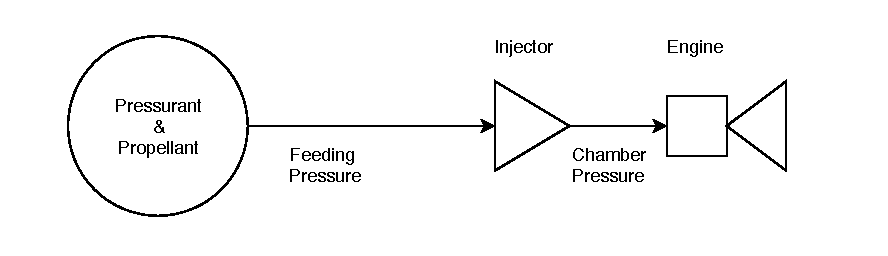
\includegraphics[width=\linewidth]{figures/blowdown_sketch}
	\caption{Simplified view of a pressure blow down system used to transport propellant to the engine. The pressurant and the propellant are separated by a diaphram.}
	\label{fig:blowdown_system}
\end{figure}

We will assume the following injection pressure loss, since neither the chamber pressure $p_c$ nor the pressure loss at the injector $\Delta p_{\text{injector}}$ are commonly cited in propulsion system specifications.
\begin{equation}
	\Delta p_{\text{injector}} \approx \frac{1}{2}p_c 
	\label{eq:injector_loss_assumption}
\end{equation}

This will lead to an estimated chamber pressure using Equation (\ref{eq:injector_loss_assumption}) as shown in the following.
\begin{gather}
	p_{\text{feed}} = p_c + \Delta p_{\text{injector}} \\
	\rightarrow \quad p_c \approx \frac{2}{3} p_{\text{feed}}
	\label{eq:chamber_pressure_estimation}
\end{gather}

During our internet research the propulsion systems in Table \ref{tab:reference} were found. All systems use monopropellants and are used for AOCS tasks of the spacecraft. In the following we will use the \textbf{XMM Thruster} as a reference case using a feeding pressure of $p_{\text{feed}}=5.5\text{bar}-24\text{bar}$ and a nozzle expansion ratio of $\epsilon=60$.\\

\begin{table}[h!]
	\centering
	\begin{tabular}{|c|c|c|c|}
		\hline
		Case & \makecell{Chamber\\ Pressure {[}bar{]}} & Expansion Ratio & \makecell{Initial Propellant\\ Temperature {[}K{]}} \\ \hline
		XMM Thruster                      &        3.67-16         &  60   &              293.15                      \\ \hline
	\end{tabular}
	\caption{Parameters needed for NasaCEA calculations based on the reference case of the XMM thruster system.}
	\label{tab:selected_reference_case}
\end{table}

Using Equation (\ref{eq:chamber_pressure_estimation}) we can translate the feeding pressure of the XMM Thruster system to a chamber pressure of $p_{c}=3.67\text{bar}-16\text{bar}$. Furthermore, an initial propellant temperature of $20^\circ\text{C}$ was assumed for all calculations. The reference case is summarized in Table \ref{tab:selected_reference_case}.
 
% B2
\section{Propellants Comparision}
Using the parameters of the reference case in Table \ref{tab:selected_reference_case} the following green propellants in Table \ref{tab:comparison} were investigated using NASA CEA. The reaction products were set to frozen from the nozzle on outwards, to prevent further reaction in the nozzle as demanded in the task description.

\begin{table}[h]
	\centering
	\begin{tabular}{|c|c|c|}
		\hline
		Propellant & Vacuum Specific Impulse {[}s{]} & Combustion Temperature {[}K{]} \\ \hline
		LMP-103S   & 253.2 & 1864-1865  \\ \hline
		AF-M315E   & 261  & 2102-2105  \\ \hline
		H2O2, 98\% & 188   & 1225    \\ \hline     
	\end{tabular}\\
	\caption{Comparison of green propellants to the reference case. Each calculation is done using the minimum and maximum feeding pressure of the reference case. If only one result is displayed no difference was calculated between max. and min. chamber pressure.}
	\label{tab:comparison}
\end{table}

% B3
\section{Propellant Optimization}
To optimize the propellant composition of Methanol, ADN and Water a rocketCEA script was written in Python. It performs a search on a composition grid, with a step size of $1\%$ weight fraction. It iterates through all possible composition permutations. The input parameters were taken from the reference case in Table \ref{tab:selected_reference_case} using only the maximum chamber pressure. The results are discussed in the following.

\paragraph{All results}
The top figure in Figure \ref{fig:fuel_optimization_all_results} shows the result of the optimization with a maximum specific impulse in vacuum of $I_{sp}=301.43s$ using $83\%$ of Methanol, $17\%$ ADN and $0\%$ Water.

\begin{figure}[!h]
	\centering
	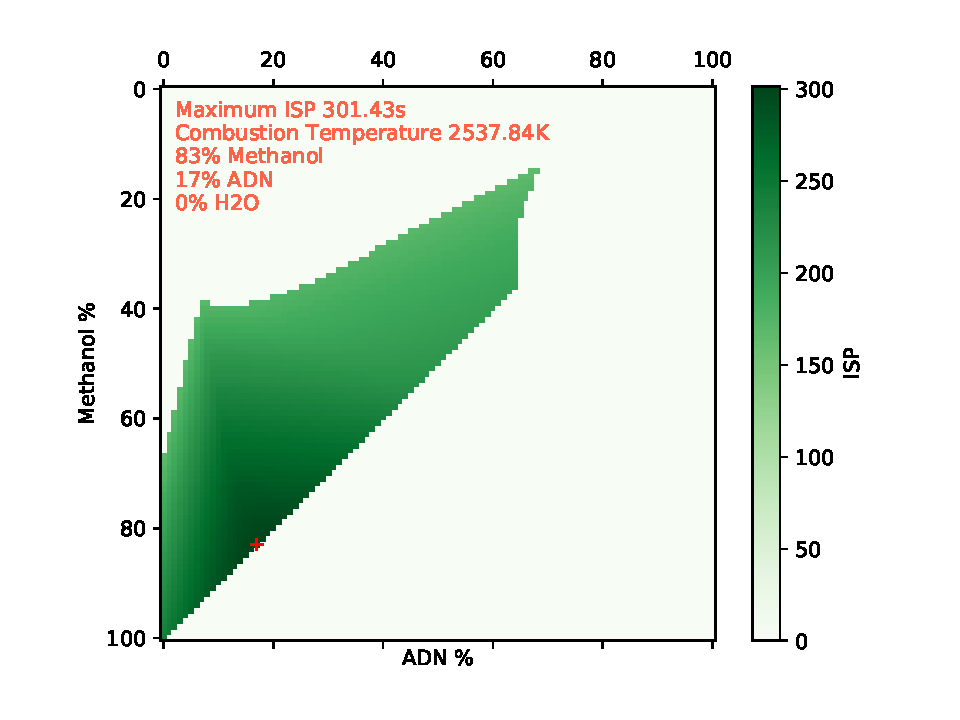
\includegraphics[width=0.8\linewidth]{figures/b3_1.pdf}
	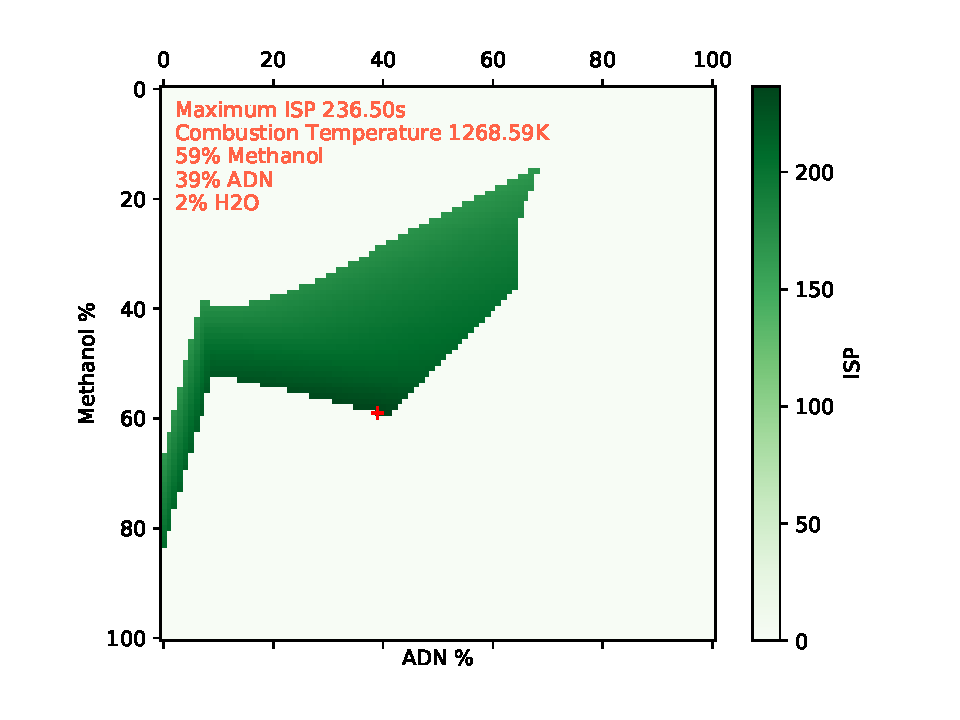
\includegraphics[width=0.8\linewidth]{figures/b3_2.pdf}
	\caption{Figure showing the fuel optimization using Nasa CEA to compute the highest possible ISP (top). The best results are highlighted with a red cross. The second figure shows the best result after all reactions with a combustion temperature above 1000$^\circ$C (1273.15K) are removed (bottom).}
	\label{fig:fuel_optimization_all_results}
\end{figure}

\paragraph{Final result}
The task demanded a combustion temperature below 1000$^\circ$C (1273.15K). Hence, all results with a higher combustion temperature were removed from the lower figure of Figure \ref{fig:fuel_optimization_all_results}. This lead to the final result with a maximum specific impulse in vacuum of $I_{sp}=236.50s$ using $59\%$ of Methanol, $39\%$ ADN and $2\%$ Water.\\

Furthermore, we need to consider that solid ADN will need to be dissolved in the other two components of the propellant. At a temperature of $20^\circ C$, which is coherent with our initial propellant temperature, $3.56$ times more Water than ADN is needed to completely dissolve the ADN. Methanol can dissolve much more ADN at a rate of only $0.86$ \cite{Larsson2011}.\\

In regard to our final result the amount of Methanol and Water is sufficient to completely dissolve the used ADN.

% B4
\section{Thruster Preliminary Design}

% B5
\section{Detailed Design Blow-Down Feed System}

% Overview
\newpage
\begin{adjustbox}{angle=90, center,caption={Overview of small propulsion systems using monopropellants.},float=table}
	\begin{tabular}{|c|c|c|c|c|c|c|}
		\hline
		Name & Propellants & \makecell{Number of\\Thrusters} & \makecell{Thruster\\Class {[}N{]}} & \makecell{Total\\Impulse [Ns]} & Other & References\\ \hline
		
		\makecell{XMM\\Thruster} & N2H4 & 8 & 20 & \makecell{$>517000$}  & \makecell{$I_{sp}=222-230s$,\\$p_{\text{feed}}=5.5-24\text{bar}$,\\$\epsilon=60$} & \makecell{ \cite{EsaXMM} \cite{ariane20N}} \\ \hline
		
		\makecell{TanDEM-X\\Thruster} & \makecell{N2H4} & 4 & 1 & \makecell{$>135000$}& \makecell{$I_{sp}=200-223s$,\\$p_{\text{feed}}=5.5-22\text{bar}$,\\$\epsilon=80$\\} & \makecell{\cite{tandemX} \cite{ariane1N}}\\ \hline
		
		\makecell{Prisma\\Thruster}& LMP-103S & 2 & 1 & \makecell{$\approx 108773$} & \makecell{$I_{sp}=204-231s$,\\$p_{\text{feed}}=4.5-22\text{bar}$,\\$\epsilon=100$} & \cite{hpgpThruster} \\ \hline
	\end{tabular}
	\label{tab:reference}
\end{adjustbox}

% References
\newpage
\printbibliography 
 
\end{document}